\documentclass[]{article}
\usepackage{lmodern}
\usepackage{amssymb,amsmath}
\usepackage{ifxetex,ifluatex}
\usepackage{fixltx2e} % provides \textsubscript
\ifnum 0\ifxetex 1\fi\ifluatex 1\fi=0 % if pdftex
  \usepackage[T1]{fontenc}
  \usepackage[utf8]{inputenc}
\else % if luatex or xelatex
  \ifxetex
    \usepackage{mathspec}
  \else
    \usepackage{fontspec}
  \fi
  \defaultfontfeatures{Ligatures=TeX,Scale=MatchLowercase}
\fi
% use upquote if available, for straight quotes in verbatim environments
\IfFileExists{upquote.sty}{\usepackage{upquote}}{}
% use microtype if available
\IfFileExists{microtype.sty}{%
\usepackage{microtype}
\UseMicrotypeSet[protrusion]{basicmath} % disable protrusion for tt fonts
}{}
\usepackage[unicode=true]{hyperref}
\hypersetup{
            pdfborder={0 0 0},
            breaklinks=true}
\urlstyle{same}  % don't use monospace font for urls
\usepackage{graphicx,grffile}
\makeatletter
\def\maxwidth{\ifdim\Gin@nat@width>\linewidth\linewidth\else\Gin@nat@width\fi}
\def\maxheight{\ifdim\Gin@nat@height>\textheight\textheight\else\Gin@nat@height\fi}
\makeatother
% Scale images if necessary, so that they will not overflow the page
% margins by default, and it is still possible to overwrite the defaults
% using explicit options in \includegraphics[width, height, ...]{}
\setkeys{Gin}{width=\maxwidth,height=\maxheight,keepaspectratio}
\IfFileExists{parskip.sty}{%
\usepackage{parskip}
}{% else
\setlength{\parindent}{0pt}
\setlength{\parskip}{6pt plus 2pt minus 1pt}
}
\setlength{\emergencystretch}{3em}  % prevent overfull lines
\providecommand{\tightlist}{%
  \setlength{\itemsep}{0pt}\setlength{\parskip}{0pt}}
\setcounter{secnumdepth}{0}
% Redefines (sub)paragraphs to behave more like sections
\ifx\paragraph\undefined\else
\let\oldparagraph\paragraph
\renewcommand{\paragraph}[1]{\oldparagraph{#1}\mbox{}}
\fi
\ifx\subparagraph\undefined\else
\let\oldsubparagraph\subparagraph
\renewcommand{\subparagraph}[1]{\oldsubparagraph{#1}\mbox{}}
\fi

% set default figure placement to htbp
\makeatletter
\def\fps@figure{htbp}
\makeatother


\date{}

\begin{document}

\emph{Ultrasuoni }

Gli ultrasuoni sono utilizzati in terapia da oltre vent' anni, anche se,
dagli studi fatti, non sono emerse grosse evidenze scientifiche riguardo
i loro effetti biologici e sulla possibilità di applicazione
terapeutica. Nonostante questo, ancora oggi più di qualcuno li utilizza.

In passato gli ultrasuoni sono stati utilizzati nella
\textbf{consolidazione delle fratture} per la loro capacità di emettere
onde di compressione e rarefazione e quindi di creare un \emph{effetto
vibratorio locale} che stimola l'osteogenesi e la riparazione tissutale
in generale, dando la possibilità agli osteoblasti di produrre e apporre
nuovo osso.

Poi sono stati sostituiti nel tempo perché si è visto che la
magnetoterapia è sicuramente più efficace.

\emph{Definizione}

Sono \textbf{vibrazioni sonore} o \emph{onde acustiche ad alte
frequenze} usate in terapia e per indagini strumentali (sonde
ecografiche, onde d'urto focalizzate); non sono percepite dall'orecchio
umano. \emph{Il metodo per ottenere gli ultrasuoni è lo stesso usato per
l\emph{'ecografia}}.

\begin{itemize}
\item
  Le \textbf{frequenze} usate in terapia variano \textbf{da 1 a 3 MHz.}
  \emph{Questo è molto significativo perché, a seconda della frequenza
  emessa, l'onda ultrasonora raggiungerà profondità diversa nei tessuti}
\item
  Le \textbf{potenze} invece sono abbastanza basse e in genere espresse
  in percentuale. Alcuni apparecchi riportano potenze di picco di 5
  Watt, ma normalmente arrivano a 3 W (\emph{alcuni strumenti con la
  testina in ceramica possono raggiungere i 4 W}). Questo anche perché
  l'ultrasuono è una \emph{termoterapia di tipo misto
  (\emph{endogena/esogena})}: la testina dell'ultrasuono si surriscalda
  e la rende una termoterapia \emph{esogena}, ma allo stesso tempo
  l'ultrasuono produce calore in profondità quindi una termoterapia
  \emph{endogena}.
\end{itemize}

\begin{quote}
Bisogna quindi considerare che aumentando la potenza dell'ultrasuono,
l'effetto termico è alto e può determinare ustioni e per questo motivo
non si riescono e non si possono utilizzare delle potenze alte.
\emph{Inoltre bisogna prestare attenzione alla regolazione della potenza
perché già a 1,5 Watt il paziente può avvertire calore locale e bisogna
evitare ustioni.}

\emph{In base alla capacità di trasformare l'energia in calore posso
distinguere \textbf{ipertermia terapia e termoterapia.} Ad esempio: la
diatermia è un'ipertermia terapia mentre gli ultrasuoni sono una
termoterapia perché riproducono un calore lieve.}
\end{quote}

\begin{itemize}
\item
  \emph{E possibile regolare anche la \textbf{modalità di trasmissione
  dell'onda di ultrasuoni:} modulata, variabile, a treni d'onda}
\end{itemize}

Ci sono degli apparecchi associati ad altri sistemi e in particolar modo
il \textbf{crioultrasuono} che permette di ridurre la componente termica
e sfruttare di più la componente meccanica e questa dà la possibilità di
utilizzarlo a \emph{potenze elevate} e, soprattutto, in \emph{fase
acuta}.

N.B. Al momento non c'è nessuna terapia strumentale che possa essere
utilizzata in fase acuta anche se alcune terapie come la tecar e la
diatermia vengono proposte \emph{perché si possono utilizzare in
atermia. }

In realtà anche a bassissima intensità viene erogato calore: non
esistono apparecchi che utilizzino la vibrazione o la corrente elettrica
senza produrre un minimo effetto termico.

Gli ultrasuoni si ottengono per e\emph{ffetto piezoelettrico} che è
legato alla capacità di alcune molecole del quarzo e di alcuni cristalli
di \emph{dilatarsi e comprimersi} emettendo vibrazioni quando sono
sottoposti ad un \emph{campo elettrico alternato}.

Dunque si utilizza un campo elettrico per mettere in vibrazione alcune
componenti e creare le onde di compressione e rarefazione. Può essere
considerato anche un effetto elettromagnetico.

Un'altra possibile applicazione terapeutica dell'ultrasuono è la
\emph{suonoforesi} cioè la possibilità di regolare la somministrazione
di alcuni farmaci attraverso l'ultrasuono.

Ci sono apparecchi, come le diatermie, che utilizzano la vibrazione per
veicolare farmaci che sono preparati preventivamente in modo tale da
avere una grandezza adatta a penetrare nei pori che vengono aperti
quando è applicata la vibrazione.

I tessuti hanno un'\emph{impedenza acustica variabile} sulla base della
quale possono assorbire, riflettere o rifrangere le onde acustiche che
lo attraversano.

\begin{itemize}
\item
  \emph{Assorbimento:} è abbastanza spiccato e riduce l'intensità
  dell'onda ultrasonora \emph{perché l'energia degli ultrasuoni si
  trasforma in calore.} L'osso ad esempio assorbe energia dieci volte
  più del muscolo
\end{itemize}

\begin{itemize}
\item
  \emph{\emph{Riflessione:}} avviene quando c'è passaggio tra due mezzi
  con diversa impendenza acustica \emph{ed è proporzionale alla
  differenza d'impendenza tra questi due mezzi} come ad esempio il
  muscolo e l'osso\emph{.}
\end{itemize}

\begin{quote}
\emph{Ad esempio gli impianti chirurgici metallici hanno diversa
impendenza rispetto al tessuto in cui sono posti per cui c'è molta
riflessioni e questo è uno dei motivi per cui il mezzo metallico può
scaldarsi maggiormente rispetto al tessuto} con ad esempio rischio di
scollamento della protesi\emph{. Oggi, però, vengono utilizzati mezzi di
sintesi inerti come il titanio che tendono difficilmente a dilatarsi e
produrre oscillazioni e dilatazioni) }
\end{quote}

\begin{itemize}
\item
  \emph{Ritrazione: si verifica quando l'onda ultrasonora attraversa due
  mezzi che hanno diversa impendenza acustica}
\end{itemize}

La \textbf{trasmissione} degli ultrasuoni attraverso i tessuti è
regolata da alcune variabili:

\begin{itemize}
\item
  Il \emph{tipo} di tessuto attraversato
\item
  \emph{\emph{Frequenza degli ultrasuoni: frequenze di 1 MH penetrano 7
  mm nel tessuto osseo, 30 mm nel muscolo, 37 mm nella cute e nel
  sottocute.}} La \emph{frequenza}, come in tutte le apparecchiature
  fisioterapiche, è quella che condiziona la capacità di
  \emph{penetrazione} dello strumento.
\item
  L'\emph{impedenza acustica} del tessuto. Ad esempio l'impedenza
  dell'osso sarà molto e alta e quella di muscolo e cute molto bassa
\end{itemize}

Gli ultrasuoni, che possono essere assorbiti o dispersi , nel momento in
cui attraversano il tessuto, producono delle \textbf{onde di
compressione e di rarefazione} (\emph{compressione/decompressione) con
movimento di va e vieni delle particelle del mezzo di trasmissione e
parallelo alla direzione delle onde di propagazione.} Si produrrà quindi
un effetto vibratorio locale con variazioni di pressione.

Sulla base di questo sono stati sviluppati gli apparecchi per le onde
d'urto che utilizzano delle pressioni molto elevate, dell'ordine di
megapascal.

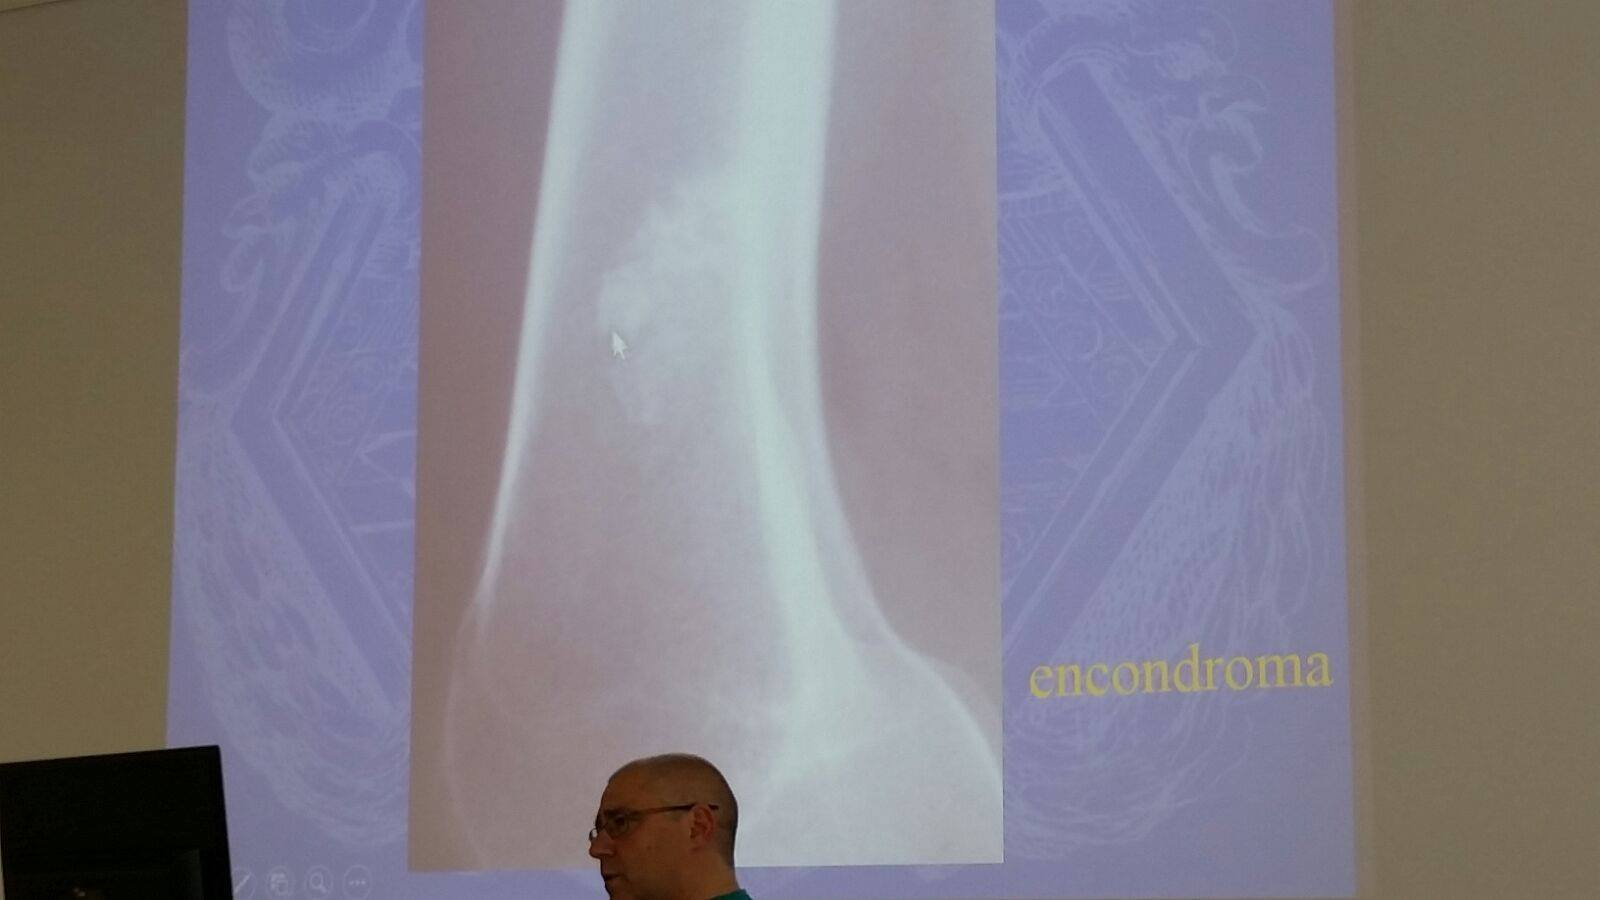
\includegraphics[width=3.92778in,height=2.38542in]{media/image1.jpeg}\textbf{Se
noi rappresentassimo graficamente un trattamento terapeutico} con
ultrasuoni, dovremmo riportare su un asse cartesiano un'onda sinusoidale
che varia in base al tempo, ma soprattutto in base alla pressione.

La \emph{pressione} che esercitiamo è legata all'intensità e quindi alla
potenza dell'apparecchio che può arrivare al massimo a 3 W.

Ma la potenza in esercizio ottimale va da 1 W a 1,5 W (già 1,8 W può
essere tollerato con difficoltà).

\emph{Caratteristiche dell'ultrasuono:}

\begin{itemize}
\item
  \textbf{Lunghezza d'onda}: la distanza tra due picchi successivi, si
  misura in nm ed è l'inverso della frequenza
\item
  \textbf{Frequenza}: numero di impulsi al secondo, si misura in Hertz
\item
  \textbf{Velocità di propagazione}: non è un parametro importante per
  l'effetto terapeutico. Dipende dal tessuto che attraversa e dalla
  densità del tessuto stesso. \emph{Vi sono diversi apparecchi che
  possono dare frequenze ben definite e vanno in applicazione modulata.}
\item
  \emph{\textbf{Densità}}
\item
  \emph{\textbf{Temperatura del mezzo}}
\item
  \emph{\textbf{Impedenza}}
\end{itemize}

\emph{Apparecchi }

Gli strumenti che emettono ultrasuoni sono costituiti da:

\begin{itemize}
\item
  Una \textbf{testina} costituita da cristalli di quarzo che vengono
  messi in vibrazione determinano l'onda ultrasonora. Oltre al quarzo
  sono usate ceramiche policristalline come il titaniato di bario o di
  piombo-zinco
\item
  Un \textbf{generatore di corrente alternata} che stimola il quarzo o i
  cristalli.
\item
  Un \textbf{cavo} che unisce il generatore alla testina emittente (in
  cui è inserito un trasduttore generalmente abbastanza grosso). Infatti
  un limite di questo apparecchio è che non si riescono a trattare le
  piccole articolazioni. Le \emph{piccole articolazioni} vengono
  trattate non per stimolazione diretta, ma con un sistema ad
  \emph{immersione in acqua} che serve per trasportare l'energia
  meccanica, la vibrazione acustica, alla zona che vogliamo trattare con
  l'interposizione dell'acqua.
\item
  Il trasduttore non viene mai applicato direttamente sula cute, ma con
  l'interposizione di un \textbf{gel} che serve per trasmette l'onda
  meccanica ed evitare che la testina si scaldi. Le case produttrici di
  questi apparecchi consigliano dei gel particolari dal punto di vista
  commerciale, come gel con sali del Mar Morto, ma non ci sono reali
  differenze tra i gel utilizzati
\item
  \emph{Il \textbf{trasduttore} può essere composto da diversi
  materiali: disco piezoelettrico, lamina di quarzo, ceramiche,
  titaniato di bario, piombo o zirconio.}
\end{itemize}

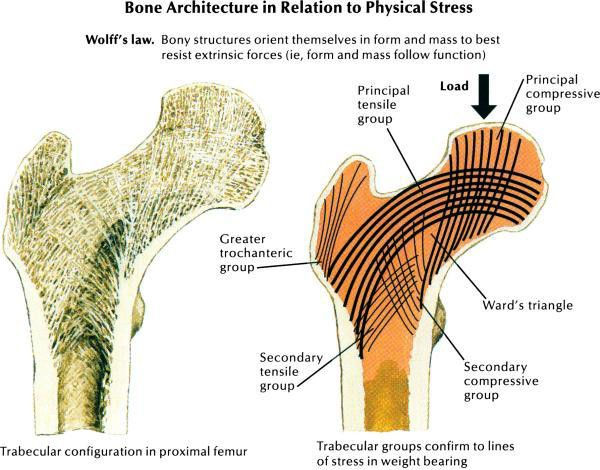
\includegraphics[width=4.16597in,height=2.69722in]{media/image2.jpeg}\emph{Questo
è un tipico apparecchio per ultrasuono carrellato che dà la possibilità
di utilizzare gli ultrasuoni in modalità continua o modulata} a 100 o 50
Hz (50 vibrazioni al secondo-pausa oppure 100 vibrazioni al
secondo-pausa), e dove si deve valutare la potenza che viene applicata.

Gli apparecchi più sofisticati e avanzati sono portatili, più piccoli e
con sistemi a led elettronici che leggono tutto direttamente. Sono
sicuramente di utilizzo più semplice.

La testina è molto grossa, ha un rivestimento con una \textbf{coppetta}
che viene riempita di gel per essere applicato direttamente sulla zona,
quindi si può fare un \textbf{trattamento fisso} di cui si può ridurre e
modulare la potenza senza utilizzare la modalità a contatto diretto
mobile.

\emph{Effetti fisiologici degli ultrasuoni}

\emph{Quando gli ultrasuoni penetrano nel corpo, l'effetto delle
vibrazioni muove tutte le particelle interne compreso il liquido
infiammatorio che viene stimolato a riassorbirsi, inoltre cedono
l'energia al tessuto che attraversano producendo calore.}

\emph{Un altro effetto provocato è l'aumento della permeabilità della
membrana cellulare che favorisce l'ingresso delle sostanze nutrienti e
l'eliminazione delle scorie.}

\emph{Nel dettaglio produce effetti:}

\begin{itemize}
\item
  \textbf{Meccanici:} Dovuti al micromassaggio esercitato
  dall'ultrasuono. Vengono applicati in modo da creare dei piccoli
  movimenti circolari e agiscono su:
\end{itemize}

\begin{itemize}
\item
  Scissione molecole complesse come le proteine e i polisaccaridi
\item
  I processi di scambio tra le cellule, accelerandoli
\item
  I processi metabolici
\item
  Il flusso ematico e linfatico, aumentandoli
\end{itemize}

\begin{quote}
L'effetto meccanico è fondamentalmente legato all' \textbf{effetto
cavitazionale} ovvero la possibilità di produrre all'interno dei tessuti
delle piccole bolle di gas che si rompono e all'interno della zona che
occupano creano delle microlesioni, delle petecchie emorragiche che
stimolano la rigenerazione tissutale e la neoangiogenesi (formazione di
nuovi vasi), formazione del tessuto di granulazione e riparazione
tissutale.
\end{quote}

\begin{itemize}
\item
  \textbf{Termici.} Tutte le elettroterapie danno un debole effetto
  termico. L'onda ultrasonora che è prodotta dalla stimolazione con
  corrente elettrica produce anch'essa un effetto termico che è
  abbastanza intenso infatti la testina si può riscaldare molto.
\item
  \textbf{Chimici.} Gli ultrasuoni possono accelerare processi chimici e
  stimolare le reazioni chimiche locali come ad esempio
  ADP-\textgreater{}ATP e tutte le reazioni che sottendono alla sintesi
  di proteine e al metabolismo produttivo.
\item
  \textbf{Neurale:}
\end{itemize}

\begin{itemize}
\item
  Agendo sulle terminazioni nervose possono \textbf{innalzare la soglia
  del dolore}. Si pensa che l'effetto sia simile a quello della TENS
  (transcutaneous electrical nerve stimulation) con \emph{gate control}
  per cui si ha inibizione degli impulsi dolorosi.
\item
  Inoltre \textbf{diminuiscono la contrattura muscolare}.
\item
  Ultimamente si è visto che a determinate intensità e pressioni elevate
  (quelle utilizzate per esempio nelle onde d'urto) possono agire anche
  sui \textbf{muscoli spastici} con effetti importanti, cosa che non è
  possibile fare con l'elettroterapia.
\end{itemize}

\emph{Dosimetria}

Vengono riportate potenze a seconda della profondità d'azione
dell'apparecchio:

\begin{itemize}
\item
  Tra i 3 e i 5 W per organi profondi (3 W sono sufficienti).
\end{itemize}

\begin{quote}
Hanno come controindicazione il \textbf{surriscaldamento} della testina
e del tessuto. Sono anche stati prodotti apparecchi con una testina che
si ghiaccia raggiungendo temperature di -3, -5 e -10 gradi
\end{quote}

\begin{itemize}
\item
  Tra 1 e 2 W sono utilizzati normalmente e l'azione è sugli organi
  superficiali e medi
\end{itemize}

Le sedute hanno durata media di 20 minuti. Il ciclo (come per tutte le
sedute di terapia strumentale) prevede 10 sedute a cadenza giornaliera.
\emph{Il tempo di applicazione è in relazione alla potenza applicata.}

\emph{Indicazioni}

Generalmente si parla di nevriti e patologie che interessano i nervi
periferici, ma in realtà hanno poco effetto.

Le indicazioni principali sono

\begin{itemize}
\item
  \emph{Affezioni del sistema nervoso (nevralgie intercostali, nevriti,
  sciatalgie, cruralgie) a ridotta intensità, al fine di
  desensibilizzare il nervo}. In questo caso si sfrutta l'effetto
  \textbf{analgesico} dovuto all'azione del calore sulle terminazioni
  nervose.
\item
  Laddove ci siano delle aderenze o fibrosi e si sfrutta l'effetto
  meccanico che permette di rendere più elastica la zona, quindi possono
  essere utilizzati in:

  \begin{itemize}
  \item
    Lesioni muscolari
  \item
    Aderenze fibrotiche post-traumatiche
  \item
    Riassorbimento di edemi post-traumatici, l'effetto delle vibrazioni
    muove tutte le particelle interne compreso il liquido infiammatorio
    che viene stimolato a riassorbirsi.
  \item
    Tendiniti
  \item
    Riacutizzazioni algiche di patologie artrosiche (gonartrosi, artrosi
    dell'arto inferiore, del piede e della caviglia, meno nelle
    coxartrosi perché non riescono a raggiungerne la profondità, sulla
    colonna vertebrale è un trattamento un po' forzato)
  \item
    Disgregazione delle calcificazioni infatti il litotrissore aveva una
    componente che utilizzava onde ultrasonore. I nuovi apparecchi non
    le usano più e sono sicuramente meno efficaci perché hanno meno
    potenza. Efficace nelle \emph{tendinopatie calcifiche della spalla}
    e nelle \emph{tendiniti rotulee} degli sportivi.
  \end{itemize}
\end{itemize}

\begin{quote}
Per andare sul sicuro nel disgregare una calcificazione si utilizzano
ormai onde d'urto perché non tutte rispondono a trattamento, dipende
dallo consistenza e dal tipo di \emph{calcificazione}: può essere di
tipo \emph{misto}, molto più resistente oppure di \emph{ossalato di
calcio} e quindi più facilmente disgregabile e di solito non occupante
lo spessore del tendine (si trova al di fuori). Se si va a rompere una
calcificazione che sta nello spessore del tendine si rischia di creare
una lesione, diminuirne la resistenza e provocarne la rottura, motivo
per cui bisogna utilizzare con cautela anche le onde d'urto.
\end{quote}

\begin{itemize}
\item
  Entesopatie
\item
  Cicatrici (specialmente quelle più rilevate e aderenti)
\item
  Morbo di Dupuytren (per l'effetto idrolitico)
\item
  Traumi contusivi e distorsivi. \emph{Ci sono studi riguardo l'utilizzo
  degli ultrasuoni per la frattura della tibia che dimostrano la
  riduzione dei tempi di consolidamento del 35-40\%, ma con un tempo di
  applicazione di 2/3 ore al giorno.}
\end{itemize}

\emph{Applicazione}

\begin{itemize}
\item
  \emph{Modalità diretta} \emph{a testina mobile}: applicato localmente
  con interposizione di gel e con movimenti circolari continui in modo
  da non mantenere l'ultrasuono fisso in una determinata zona.
\end{itemize}

\begin{quote}
Se si prende una testina di ultrasuono, si applica una potenza intorno a
0,8-1 W e si mette sulla testina dell'ultrasuono una goccia d'acqua,
l'acqua bolle, quindi c'è un riscaldamento evidente. Per quanto detto
\textbf{non} si può concentrare la testina \textbf{in un punto fisso}. È
possibile usare potenze più elevate a patto che ci sia movimento e che
non si concentri l'onda in un punto preciso.

Se invece bisogna \textbf{concentrare l'onda}, sarà necessario abbassare
l'intensità: mettiamo il \emph{gel con la coppetta} (perché c'è più gel
e assorbe di più rispetto allo strato più basso di gel che si ottiene
con il movimento). In più dobbiamo utilizzare \emph{l'applicazione
modulata} in modo che ci siano treni di onde e la pausa per non avere un
effetto surriscaldante eccessivo. Comparsa di dolore o ipertermia locale
è indice sovradosaggio (il paziente dice di sentire caldo e fastidio).
\end{quote}

\begin{itemize}
\item
  \emph{\emph{Modalità diretta a testina fissa: la testina è tenuta
  ferma da un braccio meccanico. Usata quando la zona da trattare è
  molto circoscritta, come uno sperone calcaneale}}
\item
  \emph{Trattamento a immersione} per le piccole articolazioni. Si
  utilizza un contenitore sufficientemente ampio contente acqua
  preferibilmente denaturata a 37 gradi e la testina apposta a distanza
  dalla zona di tessuto da irradiare.
\end{itemize}

\emph{Controindicazioni}

Va evitata in presenza di:

\begin{itemize}
\item
  Mezzi di sintesi metallici e protesi articolari anche se le protesi di
  ultima generazione in leghe di titanio sono meno riscaldabili. In
  questi casi si ricorre alle diatermie e alle tecarterapie che non
  arrecano danno ai mezzi di sintesi.
\item
  Gravidanza
\item
  Pacemaker
\item
  Tumori
\item
  Patologie vascolari: varici, tromboflebiti, flebotrombosi, sempre per
  l'effetto termico.
\item
  Alterazioni cutanee e della sensibilità
\item
  A livello dei bulbi oculari e aia cardiaca
\item
  \emph{Processi flogistici acuti}
\item
  \emph{Miocardiopatie}
\end{itemize}

In passato anche l'osteoporosi era considerata una controindicazione
assoluta però c'è stata una rivalutazione perché l'effetto
piezoelettrico con polarizzazione a livello del tessuto osseo potrebbe
avere azione positiva sull'osteogenesi.

\emph{IONORISONANZA CICLOTRONICA ENDOGENA (SEQEX)}

In riabilitazione i campi magnetici o elettromagnetici e il loro effetto
vibrazionale sono molto utilizzati.

La ionorisonanza ciclotronica endogena, creando campi magnetici molto
piccoli, \emph{normalizza il potenziale di membrana} per favorire gli
scambi tra tessuti intra-extra cellulari (scambi di fluidi, liquidi,
interazioni di molecole) agendo soprattutto sulle componenti polari
delle membrane.

\emph{Il moto ciclotronico del campo magnetico è così detto perché c'è
un'onda sonora che può dare un effetto di polarizzazione.}

Le membrane cellulari hanno un assetto ben definito con un proprio
potenziale di membrana. Questo potenziale tuttavia può essere
modificato: utilizzando dei codici magnetici, l'apparecchio fa una
valutazione a livello degli organi e delle loro cellule di quant'è il
valore del potenziale di membrana e ne ricava un media.

Per esempio nel fegato le cellule hanno un potenziale x e, se questo
potenziale è più basso rispetto alla valutazione dei gradi normali, si
può impostare un trattamento in quella determinata zona e l'apparecchio
ristabilisce l'equilibrio riportandolo alla normalità.

Questo crea un effetto importante, ma se parliamo di organi più
sensibili quali il cuore e il tessuto cerebrale ci possono essere degli
\textbf{effetti collaterali}: stanchezza, spossatezza, insonnia.

Il trattamento \textbf{migliora l'omeostasi cellulare}. È stato visto
che gli squilibri omeostatici sono responsabili dell'insorgenza di
diverse patologie quindi se si mantiene l'omeostasi cellulare si
mantiene l'omeostasi dell'organo.

L'effetto di questa terapia è \textbf{generalizzato}: tende a
riequilibrare gli scambi cellulari in tutto il corpo agendo su tutti i
sistemi: dal sistema immunitario all' endocrino, circolatorio, nervoso
ed osteoarticolare.

\emph{Permetterebbe potenzialmente di avere dei risultati eccezionali,
così non è.} Si può avere un effetto terapeutico in certe situazioni: i
pazienti fibromialgici possono essere astenici ed hanno un beneficio dal
trattamento perché dà iperattività (arrivano a lamentare insonnia).

Ad oggi queste apparecchiature si utilizzano poco, ma sulla base di
queste e delle microcorrenti sono state prodotte altre nuove
apparecchiature.

\emph{Metodo di applicazione}

Si sfrutta il fenomeno della risonanza.

C'è una consolle di comando pilotata da un pc che eroga terapie
attraverso delle bobine.

C'è una stuoia con fasce inserite che viene applicata su un lettino dove
il paziente si sdraia variando il decubito mentre la macchina fa un
check.

Vengono valutate diverse zone e viene fatta un'analisi; successivamente
l'operatore imposta il trattamento personalizzato per distretti
registrato su una scheda magnetica che il paziente può inserire avendo
dei benefici.

I campi elettromagnetici sono calcolati in modo utile all'organismo in
modo da variare gli effetti bioelettrici tipici del paziente. Dopo aver
prodotto queste stimolazioni elettromagnetiche che agiscono sulla
cellula, cambia il valore dell'impedenza tessutale di quell'organo e il
potenziale di membrana delle cellule. Il tutto viene poi registrato e
utilizzato.

\emph{Campi di applicazione}

Dal manuale d'uso dell'apparecchio sembrerebbe essere applicabile sulla
maggior parte delle patologie.

Molte patologie reumatiche non possono essere trattate nella fase acuta
con terapia termica o elettroterapia perché aggraverebbe un quadro di
flogosi locale come tendinite o borsite: \emph{tutte le vie strumentali
non dovrebbero essere utilizzate in acuto}.

La SEQEX invece può essere applicata in questi soggetti perché utilizza
campi a bassa intensità e l'effetto è interessante soprattutto per
articolazioni che condizionano la qualità di vita del soggetto
(ginocchio, articolazione tibiotarsica, anca, mano). Quindi con un unico
trattamento e un'unica seduta si agisce su diverse condizioni.

I \textbf{cicli} sono di dieci sedute a cadenza giornaliera, il
trattamento dura 25 minuti anticipato da un test di 5 minuti.

\emph{Effetti collaterali}

Dipendono dalla reattività e dalla condizione del paziente (possono
reagire in maniera eccessiva e positiva o tutto il contrario).

Gli effetti tipici transitori del trattamento sono: insonnia, astenia e
cefalea\emph{.}

\emph{Controindicazioni }

{[}Non sono riportare in quanto visionabili sul manuale d'uso prima di
usare l'apparecchio.{]}

Sono comunque minime per le basse intensità di azione del trattamento
(dell'ordine di microgauss).

E' da evitare in presenza di pacemaker, gravidanza, tumori.

\end{document}
